L'applicativo, oltre a seguire un design MVC, per la separazione dei componenti, implementa anche un pattern di comunicazione ad eventi, meglio conosciuto come \textit{pattern observer-delegate}. 

TODO: breve spiegazione pattern 

Nel nostro applicativo abbiamo introdotto un pattern ad eventi custom, che permettesse così di mantenere separata l'implementazione delle informazioni ottenuto da ogni singolo fragment, come si vede nella figura ~\ref{fig:ObserverForUiInformation}.
\begin{figure}[h]
	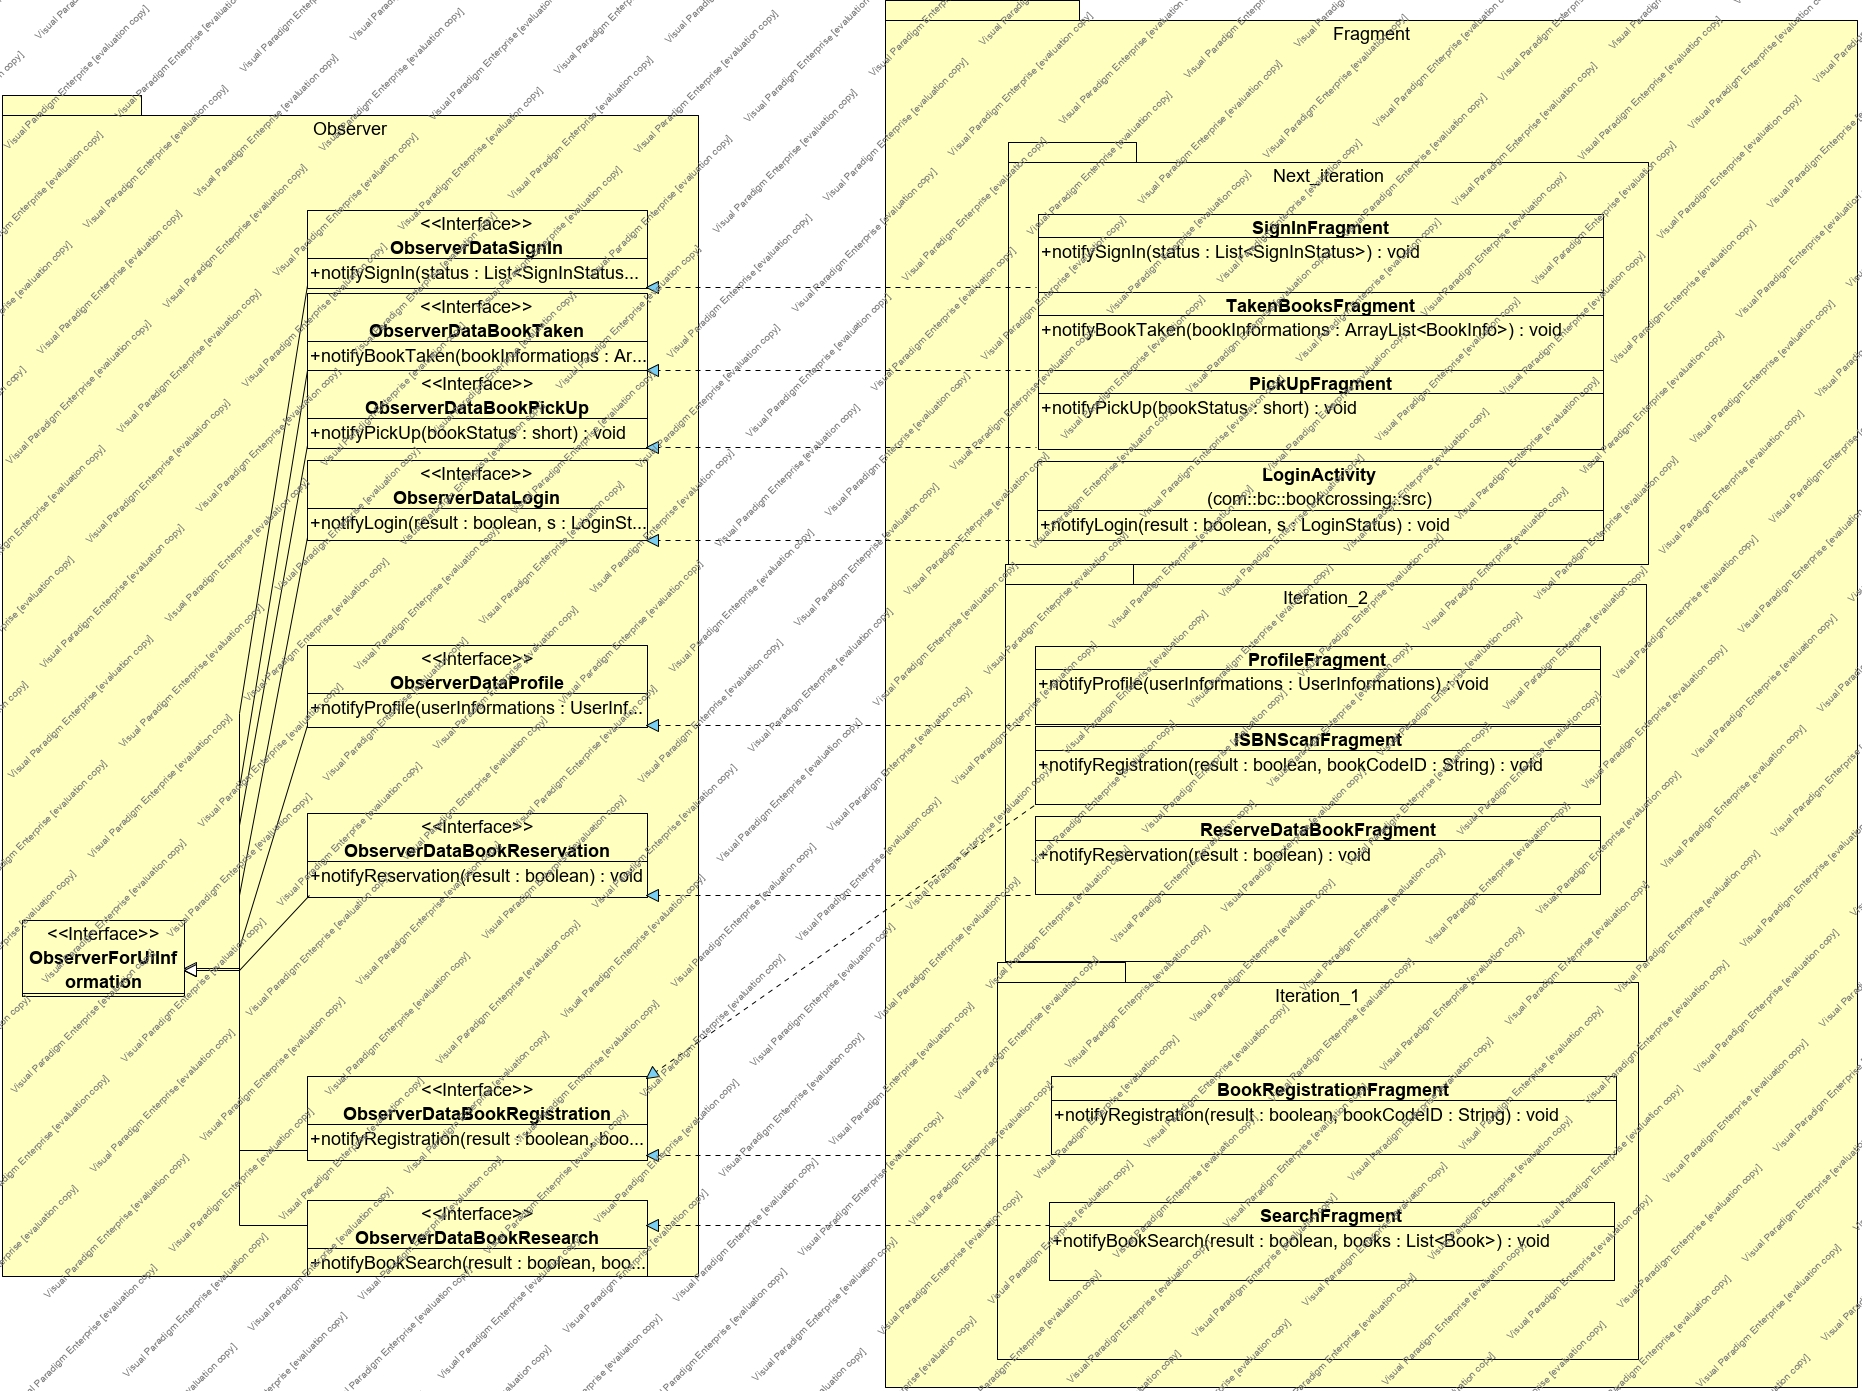
\includegraphics[width=\textwidth]{Immagini/ObserverForUIInformation}
	\caption{Interfaccie per la ricezione degli eventi}
	\label{fig:ObserverForUiInformation}
\end{figure}
Ogni singola interfaccia implementa un'interfaccia comune: questa scelta è stata adotta per rendere del tutto generico il tipo di observer che va a registrarsi per gli eventi forniti dal delegate: infatti, come si può vedere nell'interfaccia \textit{DelegateSendData} (figura ~\ref{fig:DataDispatcher}), chi è interessato ad ottenere informazioni specifiche, si registra come un oggeto di tipo \textit{ObserverForUiInformation}. Sarà poi compito del delegate fornire le corrette informazioni, richiamando le corrette callback.

\begin{figure}[h]
	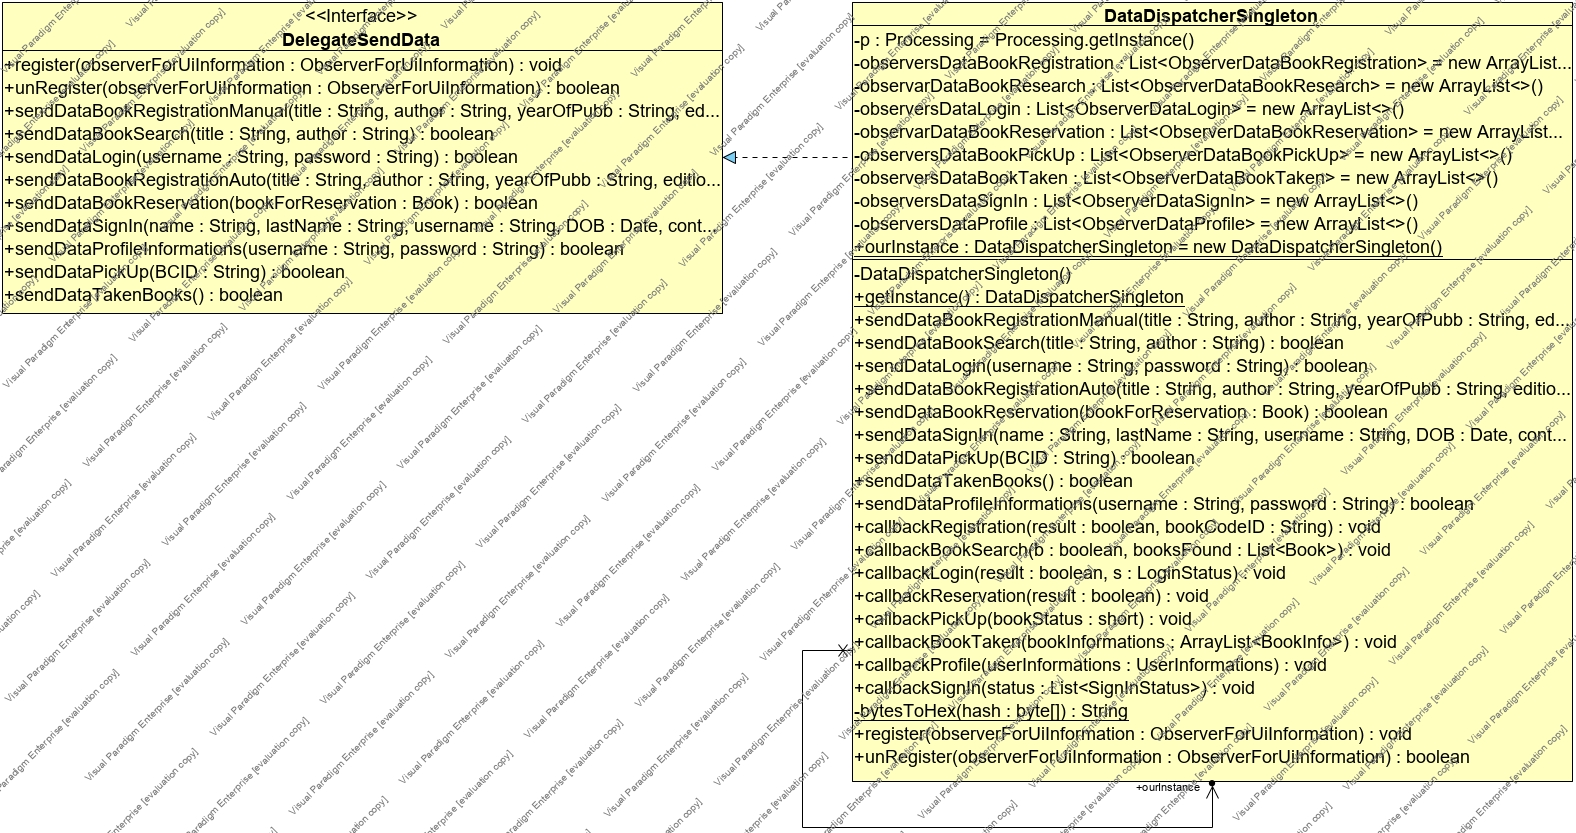
\includegraphics[width=\textwidth]{Immagini/ClassDiagramDispatcherDelegate}
	\caption{Struttura del componente \textit{DataDispatcher}}
	\label{fig:DataDispatcher}
\end{figure}

Si può quindi vedere che, nella struttura predisposta, il \textit{DataDispatcher} lavora come se fosse un \textbf{repository}, ovvero un contenitore di informazioni, che è in grado di fornire a tutti gli elementi che si registrano e che ne richiedono la ricezione.

Questi elementi, allo stadio implementativo attuale, sono rappresentati da tutti i fragment, che necessitano di ricevere/inviare informazioni per soddisfare l'interazione con l'utente: come si può notare nelle figure ~\ref{fig:LoginFragment}-~\ref{fig:LoginFragment}-~\ref{fig:BookRegistrationFragment}-~\ref{fig:PickUpFragment}-~\ref{fig:ProfileFragment}-~\ref{fig:SignInFragment}-~\ref{fig:TakenBooksFragment}, ogni singolo fragment è predisposto per ricevere le informazioni di cui ha nisogno, tramite la chiamata delle callback da parte del dispatcher stesso.

\begin{figure}[h!]
	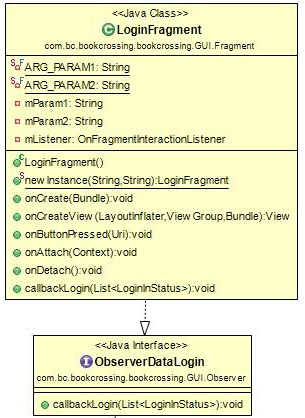
\includegraphics[width=0.5\textwidth]{Immagini/LoginFragment}
	\caption{Struttura del componente \textit{LoginFragment}}
	\label{fig:LoginFragment}
\end{figure}

\begin{figure}[h!]
	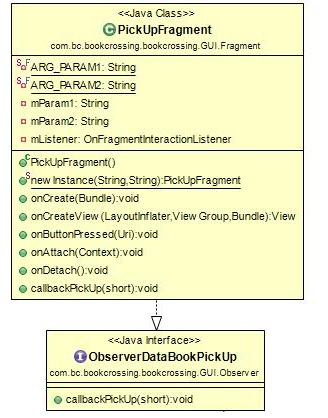
\includegraphics[width=0.5\textwidth]{Immagini/PickUpFragment}
	\caption{Struttura del componente \textit{PickUpFragment}}
	\label{fig:PickUpFragment}
\end{figure}

\begin{figure}[h!]
	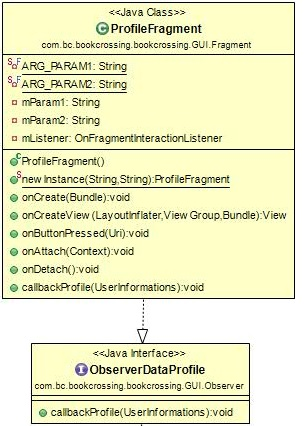
\includegraphics[width=0.5\textwidth]{Immagini/ProfileFragment}
	\caption{Struttura del componente \textit{ProfileFragment}}
	\label{fig:ProfileFragment}
\end{figure}

\begin{figure}[h!]
	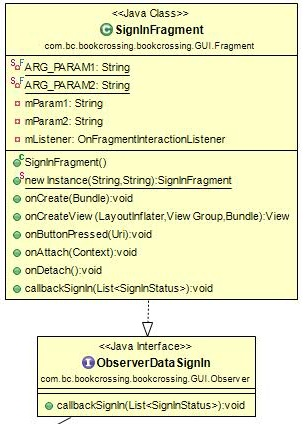
\includegraphics[width=0.5\textwidth]{Immagini/SignInFragment}
	\caption{Struttura del componente \textit{SignInFragment}}
	\label{fig:SignInFragment}
\end{figure}

\begin{figure}[h!]
	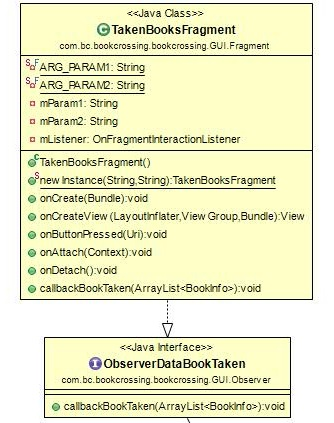
\includegraphics[width=0.5\textwidth]{Immagini/TakenBooksFragment}
	\caption{Struttura del componente \textit{TakenBooksFragment}}
	\label{fig:TakenBooksFragment}
\end{figure}

\begin{figure}[h!]
	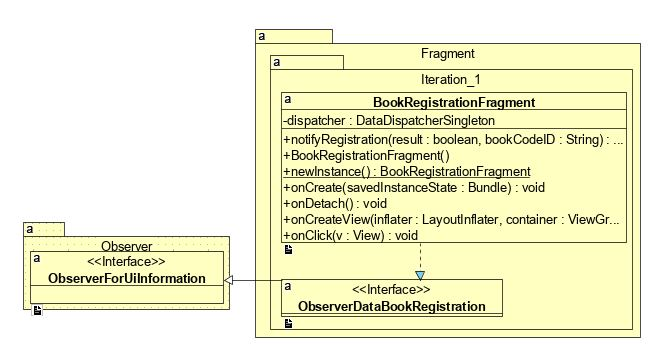
\includegraphics[width=0.5\textwidth]{Immagini/BookRegistrationFragment}
	\caption{Struttura del componente \textit{BookRegistrationFragment}}
	\label{fig:BookRegistrationFragment}
\end{figure}
